\begin{scanpage}{0038}{21}
\begin{center}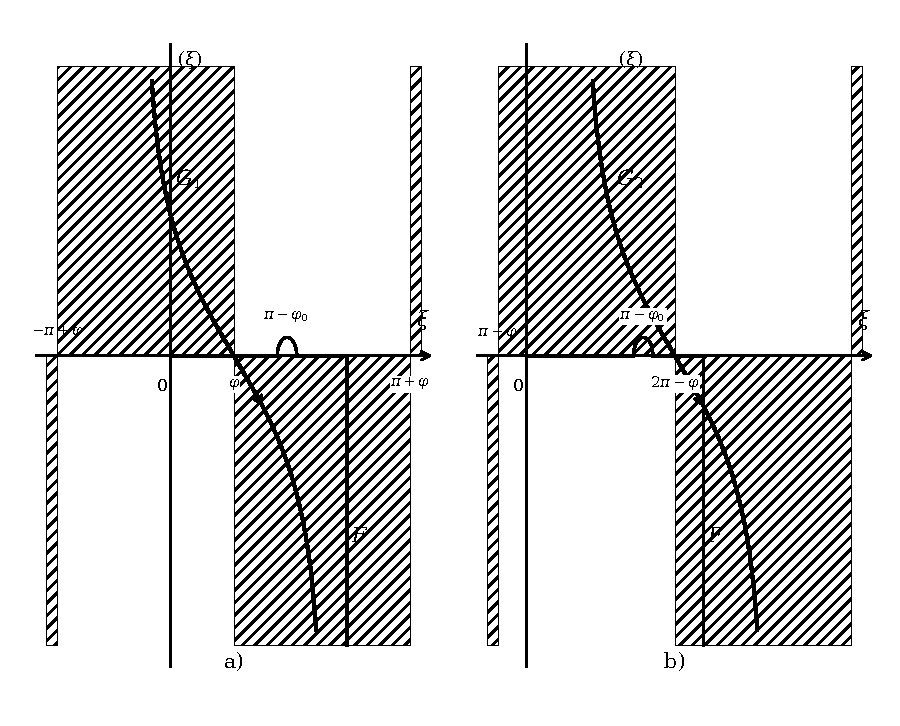
\includegraphics[width=.53\linewidth]{images/recreated/a-0038-fig7.pdf}\par Figure 7. The integration contour in Equations (3.14).\end{center}
\[I_1=\frac1{i\pi k}\int_{D_0}\frac{e^{ikr\cos\zeta}\,d\zeta}{\cos\phi_0+\cos(\zeta-\phi)}+\begin{cases}0&\text{with }\phi<\pi+\phi_0,\\\dfrac2{k\sin\phi_0}e^{-ikr\cos(\phi-\phi_0)}&\text{with }\phi>\pi+\phi_0,\end{cases}\tag{3.17}\]
if $\phi>\pi$. The integration contour $D_0$ is shown in Figure 4.

By means of Equation (3.06) and the equality
\[E_z=ikA_z,\tag{3.18}\]
let us find the field which is radiated by the uniform part of the current excited on the face $\phi=0$ by the plane wave (1.23)
\[\frac{E_z}{E_{0z}}=\begin{cases}v_1^+(\phi,\phi_0)-e^{-ikr\cos(\phi+\phi_0)}&\text{with }0<\phi<\pi-\phi_0,\\v_1^+(\phi,\phi_0)&\text{with }\pi-\phi_0<\phi<\pi,\\v_1^-(\phi,\phi_0)&\text{with }\pi<\phi<\pi+\phi_0,\\v_1^-(\phi,\phi_0)-e^{-ikr\cos(\phi-\phi_0)}&\text{with }\pi+\phi_0<\phi<\alpha,\end{cases}\tag{3.19}\]
\end{scanpage}
